
\section{代数间奏二：Lying Over 与\trNakayama{}引理}

\epigraph
  {代数是魔鬼开给数学家的价码。魔鬼说：我会把这台威力强大的机器送给你，
   你喜欢的任何问题它都能回答。你唯一要付出的，是把灵魂交给我：放弃几何，
   这台奇妙的机器便归你所有。}
  {——M.~\trAtiyah，[At2, p.~659]；另请参看 \S0.3 篇首的\trAtiyah{}引语}

为给下一节关于\trIntegral\trMorphism{}的讨论作好铺垫，我们先发展几条代数上的预备知识。我们所用的一个巧招，还可以用来证明\trNakayama{}引理，所以我们对此也一并讨论。

设 $\phi\colon B\to A$ 是一个\trRingMorphism。若 $a\in A$ 满足某条\trMonicPolynomial{}（monic polynomial）%
\[
a^n+?a^{n-1}+\cdots+?=0
\]
其中诸系数落在 $\phi(B)$ 中，就称 $a$ \textbf{在 $B$ 上\trIntegral}（integral over $B$）。若环\emph{映射} $\phi\colon B\to A$ 使得 $A$ 的每个元素都在 $\phi(B)$ 上\trIntegral，就称 $\phi$ 是\textbf{\trIntegral{}的}（integral）。一个\trIntegral{}的环映射 $\phi$，若还是环的\emph{包含映射}，便称为一个\textbf{\trIntegralExtension{}}（integral extension）。%
你应当把\trIntegral{}映射与\trIntegralExtension{}，看作「\trAlgebraic\trFieldExtension」这一概念的环论推广。

\begin{exercise}\label{ex:integrality-affine-cover}
证明：若 $\phi\colon B\to A$ 是\trRingMorphism{}，$(b_1,\dots,b_n)=1$ 于 $B$ 中，且对一切 $i$，$B_{b_i}\to A_{\phi(b_i)}$ 都是\trIntegral{}的，则 $\phi$ 是\trIntegral{}的。提示：把 $B$ 换成 $\phi(B)$，化归到 $B$ 是 $A$ 的\trSubring{}的情形。设 $a\in A$。证明：存在与 $i$ 无关的某对 $t$ 与 $m$，使得 $b_i^t a^m\in B+Ba+Ba^2+\cdots+Ba^{m-1}$。再循\cref{thm:sheaf-on-distinguished-base}证明中的「\trPartitionOfUnity」式论证，证明 $a^m\in B+Ba+Ba^2+\cdots+Ba^{m-1}$。
\end{exercise}

\begin{exercise}\label{ex:integrality-localization-quotient}
\begin{enumerate}[label=(\alph*)]
\item 证明：\emph{映射} $\phi\colon B\to A$ 为\trIntegral{}的这一性质，对 $B$ 作\trLocalization{}与取\trQuotient、以及 $A$ 取\trQuotient，总是保持；但对 $A$ 作\trLocalization{}则不然。更精确地：设 $\phi$ 是\trIntegral{}的。证明：所诱导的映射 $T^{-1}B\to\phi(T)^{-1}A$、$B/J\to A/\phi(J)A$ 与 $B\to A/I$ 都是\trIntegral{}的（其中 $T$ 是 $B$ 的一个\trMultiplicativeSubset，$J$ 是 $B$ 的一个\trIdeal，$I$ 是 $A$ 的一个\trIdeal），但 $B\to S^{-1}A$ 未必\trIntegral（其中 $S$ 是 $A$ 的一个\trMultiplicativeSubset）。（后者的提示：证明 $k[t]\to k[t]$ 是\trIntegral{}的环映射，但 $k[t]\to k[t]_{(t)}$ 不是。）
\item 证明：是整\emph{扩张}这一性质，对 $B$ 作\trLocalization{}保持，但对 $A$ 作\trLocalization{}或取\trQuotient{}都不保持。（后者的提示：$k[t]\to k[t]$ 是\trIntegralExtension{}，但 $k[t]\to k[t]/(t)$ 不是。）
\item 事实上，$\phi$ 是整\emph{扩张}（相对于\trIntegral{}的\emph{映射}）这一性质，连对 $B$ 取\trQuotient{}也不保持。（取 $B=k[x,y]/(y^2)$ 与 $A=k[x,y,z]/(z^2,xz-y)$，则 $B$ 单射入 $A$，但 $B/(x)$ 不单射入 $A/(x)$。）不过在某些情形它确实保持。设 $\phi\colon B\to A$ 是\trIntegralExtension{}，而 $J\subset B$ 是某个\trIdeal{} $I\subset A$ 的\trRestriction{}。（旁注：你可以证明，当 $J$ 为\trPrimeIdeal{}时这条成立。）证明：所诱导的映射 $B/J\to A/JA$ 是\trIntegralExtension{}。（提示：证明复合映射 $B/J\to A/JA\to A/I$ 是\trInjectiveMap。）
\end{enumerate}
\end{exercise}

下面这条引理会用一个有用却略带刁滑的小招。

\textbf{8.2.1.\ \trhLemma{}。}\ ——\ \emph{设 $\phi\colon B\to A$ 是一个\trRingMorphism。则 $a\in A$ 在 $B$ 上\trIntegral，当且仅当它含于 $A$ 的某个\trSubalgebra{}（subalgebra），且该\trSubalgebra{}是一个有限生成的 $B$-\trModule。}%

\emph{证明。}\ 若 $a$ 满足一条 $n$ 次的\trMonicPolynomial{}方程，那么 $A$ 的由 $1,a,\dots,a^{n-1}$ 生成的那个 $B$-\trSubmodule{}对乘法封闭，从而是 $A$ 的一个\trSubalgebra{}。

反之，设 $a$ 含于 $A$ 的某个\trSubalgebra{} $A'$，而后者是一个有限生成的 $B$-\trModule。取定 $A'$（作为 $B$-\trModule）的一组有限生成元 $\mathsf{m}_1,\dots,\mathsf{m}_n$。于是存在诸 $b_{ij}\in B$，使得 $a\mathsf{m}_i=\sum_j b_{ij}\mathsf{m}_j$。这样便有
\begin{equation*}\tag{8.2.1.1}\label{eq:adjugate-trick-matrix}
\bigl(a\,\mathrm{Id}_{n\times n}-[b_{ij}]_{ij}\bigr)
\begin{pmatrix}\mathsf{m}_1\\ \vdots\\ \mathsf{m}_n\end{pmatrix}
=
\begin{pmatrix}0\\ \vdots\\ 0\end{pmatrix},
\end{equation*}
其中 $\mathrm{Id}_n$ 是 $A$ 中的 $n\times n$ 单位矩阵。矩阵 $\bigl(a\,\mathrm{Id}_{n\times n}-[b_{ij}]_{ij}\bigr)$ 无法求逆，但差一点就能。回想：$n\times n$ 矩阵 $M$ 带有一个\emph{\trAdjugateMatrix{}}（adjugate matrix）$\mathrm{adj}(M)$，满足 $\mathrm{adj}(M)M=\det(M)\mathrm{Id}_n$（$\mathrm{adj}(M)$ 的第 $(i,j)$ 个元素，是从 $M$ 中删去第 $i$ 列与第 $j$ 行所得矩阵的行列式再乘以 $(-1)^{i+j}$。你多半已以「逆矩阵存在时 $M^{-1}$ 的公式」的面貌见过它；例如参看 [DF, p.~440]。）$\mathrm{adj}(M)$ 的元素是 $M$ 的元素的多项式。用 $\mathrm{adj}\bigl(a\,\mathrm{Id}_{n\times n}-[b_{ij}]_{ij}\bigr)$ 乘 \eqref{eq:adjugate-trick-matrix}，便得
\[
\det\bigl(a\,\mathrm{Id}_{n\times n}-[b_{ij}]_{ij}\bigr)
\begin{pmatrix}\mathsf{m}_1\\ \vdots\\ \mathsf{m}_n\end{pmatrix}
=
\begin{pmatrix}0\\ \vdots\\ 0\end{pmatrix}.
\]
于是 $\det(aI-[b_{ij}])$ 零化了诸生成元 $\mathsf{m}_i$，从而零化 $A'$ 的每个元素，也就是说 $\det(aI-[b_{ij}])=0$。而把行列式展开，便得到 $a$ 的一个系数落在 $B$ 中的\trIntegrality{}方程。\hfill$\square$

\textbf{8.2.2.\ \trhCorollary{}（有限蕴含\trIntegral）。}\ ——\ \emph{若 $A$ 是一个有限 $B$-\trAlgebra（即一个有限生成的 $B$-\trModule），则 $\phi$ 是一个\trIntegral{}的环映射。}

逆命题不真：\trIntegral{}推不出有限，因为 $\mathbb{Q}\hookrightarrow\overline{\mathbb{Q}}$ 是\trIntegral{}的环映射，而 $\overline{\mathbb{Q}}$ 不是有限的 $\mathbb{Q}$-\trModule。（\trFieldExtension{}是\trIntegral{}的，若它是\trAlgebraic{}的。）

\begin{exercise}\label{ex:integrality-composition}
证明：若 $C\to B$ 与 $B\to A$ 都是\trIntegral{}的环映射，则它们的\trComposition{}也是。
\end{exercise}

\begin{exercise}\label{ex:integral-elements-subalgebra}
设 $\phi\colon B\to A$ 是一个\trRingMorphism。证明：$A$ 中在 $B$ 上\trIntegral{}的那些元素构成 $A$ 的一个\trSubalgebra{}。
\end{exercise}

\textbf{8.2.3.\ \trhRemark{}：超越理论。}\quad 这些想法引出了\emph{超越理论}（transcendence theory）的若干主要事实，即我们讨论簇的\trDimension{}时所需要的那一批；见练习／定义~12.2.A。%

\textbf{8.2.4.\ Lying Over 定理与 Going-Up 定理。}\quad Lying Over 定理是\trIntegralExtension{}的一条有用的性质。

\textbf{8.2.5.\ Lying Over 定理。}\ ——\ \emph{设 $\phi\colon B\to A$ 是一个\trIntegralExtension{}。则对任意\trPrimeIdeal{} $\mathfrak{q}\subset B$，存在\trPrimeIdeal{} $\mathfrak{p}\subset A$ 使得 $\mathfrak{p}\cap B=\mathfrak{q}$。}

把这套假设有多弱说个明白：$B$ 不必\trNoetherian，$A$ 也不必在 $B$ 上\trFinitelyGenerated。

\textbf{8.2.6.}\ \emph{几何翻译：若 $B\to A$ 是\trIntegralExtension{}，则 $\Spec A\to\Spec B$ 是满的。}\quad 尽管 Lying Over 定理~8.2.5 是一条代数定理，这个名字却可以作几何解读：该定理断言，相应的概形间的\trMorphism{}是满的。（概形间的映射称为\textbf{满}（surjective），如果其底下的集合映射是\trSurjectiveMap。）%
翻译过来就是：「楼下」的每个素理想 $\mathfrak{q}$ 的「上方」，都有一个素理想 $\mathfrak{p}$；见图~\ref{fig:lying-over-picture}。（正因如此，若 $\mathfrak{p}\cap B=\mathfrak{q}$，人们便常说 $\mathfrak{p}$「位于 $\mathfrak{q}$ 之上」。）

\begin{figure}[htbp]
\centering
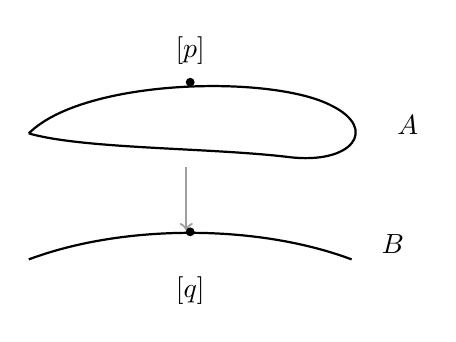
\begin{tikzpicture}[scale=1.0,line width=0.8pt]
  \draw (-2.0,1.25)
        .. controls (-1.3,1.95) and (1.1,2.0) .. (1.85,1.6)
        .. controls (2.45,1.3) and (2.1,0.85) .. (1.3,0.95)
        .. controls (0.3,1.07) and (-1.3,1.05) .. (-2.0,1.25);
  \fill (0.05,1.9) circle (1.6pt);
  \node at (0.05,2.3) {$[\mathfrak{p}]$};
  \node[anchor=west] at (2.55,1.35) {$\Spec A$};
  \draw[gray!75,->] (0,0.82) -- (0,0.02);
  \draw (-2.0,-0.35) .. controls (-0.8,0.1) and (0.9,0.1) .. (2.1,-0.35);
  \fill (0.05,0.0) circle (1.6pt);
  \node[anchor=west] at (2.35,-0.15) {$\Spec B$};
  \node at (0.05,-0.75) {$[\mathfrak{q}]$};
\end{tikzpicture}
\caption{Lying Over 定理~8.2.5 的一幅图：若 $\phi\colon B\to A$ 是\trIntegralExtension{}，则 $\Spec A\to\Spec B$ 是满的。（依原书手绘图重绘。）}\label{fig:lying-over-picture}
\end{figure}

下面这道练习为证明作好了准备。

\begin{exercise}[\hard]\label{ex:integral-field-case}
证明：$A$ 是\trField{}时的特例可以翻译为：若 $B\subset A$ 是\trSubring{}而 $A$ 在 $B$ 上\trIntegral，则 $B$ 是\trField。请证明它。（提示：你必须证明 $B$ 中一切非零元素都在 $B$ 中有\trInverseElement。这里是一个开头：若 $b\in B$，则 $1/b\in A$，而它满足某条在 $B$ 上的\trIntegrality{}方程。）
\end{exercise}

\emph{\hard\ Lying Over 定理~8.2.5 的证明。}\ 我们先作一个归约：对 $\mathfrak{q}$ 作\trLocalization{}（\trIntegrality{}由\cref{ex:integrality-localization-quotient}(b) 得以保持），便可假设 $(B,\mathfrak{q})$ 是一个\trLocalRing。然后任取 $A$ 的一个\emph{极大}理想 $\mathfrak{p}$。考虑如下的图。
\[
\begin{tikzcd}[row sep=3em, column sep=4.2em]
A \ar[r] & A/\mathfrak{p} & \text{域} \\
B \ar[u, hook] \ar[r] & B/(\mathfrak{p}\cap B) \ar[u, hook] &
\end{tikzcd}
\]
右边的竖直箭头由\cref{ex:integrality-localization-quotient}(c) 知是一个\trIntegralExtension{}。由\cref{ex:integral-field-case}，$B/(\mathfrak{p}\cap B)$ 也是\trField，于是 $\mathfrak{p}\cap B$ 是\trMaximalIdeal，从而它就是 $\mathfrak{q}$。\hfill$\square$

\begin{exercise}[重要练习（\textbf{Going-Up} 定理）]\label{ex:going-up-theorem}
\begin{enumerate}[label=(\alph*)]
\item 设 $\phi\colon B\to A$ 是一个\trIntegral{}的环\emph{映射}（不必是\trIntegralExtension{}）。证明：若 $\mathfrak{q}_1\subset\mathfrak{q}_2\subset\cdots\subset\mathfrak{q}_n$ 是 $B$ 的素理想的一条链，而 $\mathfrak{p}_1\subset\cdots\subset\mathfrak{p}_m$ 是 $A$ 的素理想的一条链，使得诸 $\mathfrak{p}_i$「位于」诸 $\mathfrak{q}_i$ 之上（且 $1\le m<n$），则第二条链可以扩充成 $\mathfrak{p}_1\subset\cdots\subset\mathfrak{p}_n$，使得这一情形依然成立。（提示：先化归到 $m=1$、$n=2$ 的情形；再化归到 $\mathfrak{q}_1=(0)$ 与 $\mathfrak{p}_1=(0)$ 的情形；然后使用 Lying Over 定理~8.2.5。）
\item 给这条定理画一幅图（与图~\ref{fig:lying-over-picture} 相仿）。
\end{enumerate}
\end{exercise}

也有与它们类似的「Going-Down」型结果（所需的假设颇为不同）；例如参看定理~12.2.12 与\mbox{练习~24.5.E}。

\textbf{8.2.7.\ \trNakayama{}引理。}

引理~8.2.1 证明中的那个巧招，还可以用来很快地证明\trNakayama{}引理——往后我们会一用再用。这个名字被用来称呼好几个互不相同却彼此相关的结果，我们在此一一讨论。（几何解读将在\mbox{练习~14.3.D}中给出。）趁这个巧招在我们脑中还热乎，不妨顺手把它证掉。

\textbf{8.2.8.\ \trNakayama{}引理版本~1。}\ ——\ \emph{设 $A$ 是一个环，$I$ 是 $A$ 的一个\trIdeal，$M$ 是一个有限生成的 $A$-\trModule，满足 $M=IM$。那么存在 $a\in A$，$a\equiv 1\pmod{I}$，使得 $aM=0$。（等价地：存在某个 $i\in I$，用 $i$ 作乘法在 $M$ 上诱导的是恒等映射：对一切 $m\in M$ 有 $im=m$。）}

\emph{证明。}\ 设 $M$ 由 $\mathsf{m}_1,\dots,\mathsf{m}_n$ 生成。那么由于 $M=IM$，存在诸 $a_{ij}\in I$ 使得 $\mathsf{m}_i=\sum_j a_{ij}\mathsf{m}_j$。于是
\begin{equation*}\tag{8.2.8.1}\label{eq:nakayama-adjugate-matrix}
(\mathrm{Id}_n-Z)
\begin{pmatrix}\mathsf{m}_1\\ \vdots\\ \mathsf{m}_n\end{pmatrix}
=0,
\end{equation*}
其中 $Z=(a_{ij})$。用 $\mathrm{adj}(\mathrm{Id}_n-Z)$ 左乘 \eqref{eq:nakayama-adjugate-matrix} 的两边，便得
\[
\det(\mathrm{Id}_n-Z)
\begin{pmatrix}\mathsf{m}_1\\ \vdots\\ \mathsf{m}_n\end{pmatrix}
=0.
\]
但当你把 $\det(\mathrm{Id}_n-Z)$ 展开时，由于 $Z$ 的元素都落在 $I$ 中，你得到的会是某个模 $I$ 同余于 $1$ 的东西。\hfill$\square$

说说你为什么要在意它。设 $I$ 含于 $A$ 的全部\trMaximalIdeal{}。（全体\trMaximalIdeal{}之交称为\textbf{\trJacobsonRadical{}}（Jacobson radical），但我们不会使用这个说法。作为对照，回想\trNilradical{}是 $A$ 的诸\emph{\trPrimeIdeal}之交。）%
此时，任何 $a\equiv 1\pmod{I}$ 都是可逆的。（此刻我们还没用上\trNakayama{}引理！）理由：否则 $(a)\neq A$，于是\trIdeal{} $(a)$ 含于某个\trMaximalIdeal{} $\mathfrak{m}$——但 $a\equiv 1\pmod{\mathfrak{m}}$，矛盾。既然 $a$ 可逆，我们便有下述结果。

\textbf{8.2.9.\ \trNakayama{}引理版本~2。}\ ——\ \emph{设 $A$ 是一个环，$I$ 是 $A$ 的一个含于全部\trMaximalIdeal{}的\trIdeal，$M$ 是一个有限生成的 $A$-\trModule。（最有趣的情形是 $A$ 为\trLocalRing{}而 $I$ 为其\trMaximalIdeal{}的情形。）设 $M=IM$。那么 $M=0$。}

\begin{exercise}[\trNakayama{}引理版本~3]\label{ex:nakayama-version-3}
设 $A$ 是一个环，$I$ 是 $A$ 的一个含于全部\trMaximalIdeal{}的\trIdeal。设 $M$ 是一个\emph{有限生成}的 $A$-\trModule，而 $N\subset M$ 是一个\trSubmodule。若 $N/IN\to M/IM$ 是\trSurjectiveMap，则 $M=N$。
\end{exercise}

\begin{exercise}[重要练习（\trNakayama{}引理版本~4：$M/\mathfrak{m}M$ 的生成元可提升为 $M$ 的生成元）]\label{ex:nakayama-version-4}
设 $(A,\mathfrak{m})$ 是一个\trLocalRing。设 $M$ 是一个有限生成的 $A$-\trModule，而 $f_1,\dots,f_n\in M$，使得（诸 $f_i$ 的像）生成 $M/\mathfrak{m}M$。那么 $f_1,\dots,f_n$ 生成 $M$。（特别地，取 $M=\mathfrak{m}$：只要有了 $\mathfrak{m}/\mathfrak{m}^2$ 的一组生成元，它们也就生成 $\mathfrak{m}$。）
\end{exercise}

\begin{exercise}[推广引理~8.2.1 的重要练习]\label{ex:integrality-faithful-module}
回想：若 $B$ 中在 $N$ 上以恒等映射作用的元素仅有 $1$（等价地，$B$ 中在 $N$ 上以零映射作用的元素仅有 $0$），就称 $B$-\trModule{} $N$ 是\textbf{\trFaithful{}的}（faithful）。设 $S$ 是环 $A$ 的一个\trSubring，$r\in A$。设存在一个\trFaithful{}的 $S[r]$-\trModule{} $M$，它作为 $S$-\trModule{}是有限生成的。证明：$r$ 在 $S$ 上\trIntegral。（提示：把\trNakayama{}引理版本~1（引理~8.2.8）的证明改动几个词。）
\end{exercise}

\begin{exercise}\label{ex:integral-closure-integrally-closed}
设 $A$ 是一个\trIntegralDomain，而 $\widetilde{A}$ 是 $A$ 在 $\mathrm{K}(A)$ 中的\textbf{\trIntegralClosure}，即 $\mathrm{K}(A)$ 中那些在 $A$ 上\trIntegral{}的元素——由\cref{ex:integral-elements-subalgebra}，它们构成一个\trSubalgebra{}。证明：$\widetilde{A}$ 在 $\mathrm{K}(\widetilde{A})=\mathrm{K}(A)$ 中是\trIntegrallyClosed{}的。
\end{exercise}
